\chapter[]{Introduction to the security of ICT systems}

\section{Why is security important}
There are many angles to answer this question:
\begin{itemize}
    \item \textbf{People}: we want to protect our assets (money, data, etc.), confidentiality/privacy (identity), physical safety, and so on.

    \item \textbf{Countries/governments}: they need to protect the nation’s safety and interests (critical infrastructures, health, geo-political decisions, military (communication and data). Also, efficient \& secure communication (e.g., citizens and public entities) is needed.

    \item \textbf{Companies} and \textbf{organizations}: they need to protect assets and resources (services, data, etc.) in order to maintain a successful businesses (intellectual property).
\end{itemize}

Example case of why security is important: the 2007 attack on T.J. Maxx supermarkets in the USA (hackers intercepted the communication between the supermarkets and the banks, which was on an unsafe protocol), 45.7 M credit and debit cards got their data stolen.

Other examples:
\begin{itemize}
    \item Nowadays, investing is popular, and a significant portion of investing is done on cryptocurrencies, so their safety is paramount, or people will lose their money.

    \item On February 23, 2021, a massive data breach regarding nearly 500.000 people was revealed in the press, involving the company Dedalus Biologie. The name, first name, social security number of people were exposed, together with all their medical information, often sensitive (HIV, cancers, pregnancies, and so on).

    \item In general, data breaches like the one just described are more common than we think: in 2022, there were about 420 million victims (\href{https://www.idtheftcenter.org/publication/2022-data-breach-report/}{source}).

    \item Smart Locks of homes and electric vehicles: these things can all be hacked, resulting in significant danger! Modern cars can even be remotely operated by hackers. As \textbf{robotics} makes more and more progress, the threat of hacking becomes more and more serious.

    \item A nation's critical infrastructures can be hacked, leading to significant damage. The energy sector received more cyber attacks in 2022 than ever before, and these attacks can knock down internet communications systems and other necessary infrastructures. We'll study the motivations behind these attacks.

    \item As we said, companies want to protect their assets. Companies lose tens of \textbf{billions} of dollars yearly for ransomware attacks, but more importantly, organizations face business downtime, reputational damage and diminished customer trust.
\end{itemize}

\section{What is computer/information security?}
Security evolved over time. Before computers, security was about protecting some physical place (like a bank) that contained valuable things.

Then, computers arrived, and the first model was a \textbf{centralized} one: a central mainframe (server) placed in a protected location/dedicated room. All data and processing was concentrated in the mainframe, and there was restricted access to the room (only administrators).

The centralized access could be done in 2 ways:
\begin{itemize}
    \item Direct access - through punched cards
    \item Remote access - done mainly from 'stupid' terminals (only keyboard and screen, no memory and no CPU) via unicast (one line per terminal) communication over end-to-end dedicated lines.
\end{itemize}
Then, we moved to the distributed model, when internet started growing. This model is characterized by distributed processing, storage, and control, with (initially) \textbf{trusted} nodes distributed in different locations, connected through 'broadcast' communication (shared, not unicast) and/or shared communication lines, and dedicated equipments (gateways).

In this model, terminals had (low) processing and memory capabilities, and nodes were communicating through network protocols (IP, TCP, etc.).

Nowadays, we have highly distributed systems, with various types of nodes: PCs, data servers, network equipments, smartphones, embedded systems (cars, home appliances), IoT, etc. They can have large or low resources (networking, CPUs and GPUs, memory). These nodes are connected through different types of communication lines: wired, wireless, satellite. Many network protocols are used, even if many of them were originally defined for closed or trusted environments (IP, TCP, UDP, DHCP, ICMP, ARP, etc.). These protocols can be exploited to perform attacks.

\paragraph{Definitions of security}
The definition of security depends on the era.
\begin{itemize}
    \item In the centralized model, security was:
    \begin{itemize}
        \item Physical protection:
        \begin{itemize}
            \item Protection of the main center: keep it a safe location, impede vandalism, unauthorized (physical) access from persons, provide constant cooling and electricity.

            \item Protection of the communication lines: protect the cables and devices involved (e.g. concentrator)
        \end{itemize}

        \item Logical protection (typically weak): authentication (with username and password) and authorization (what operations can each class of users do). The mainframe's OS had to support the basic security services: authentication and authorization.
    \end{itemize}

    \item In the decentralized model, security became more an issue of keeping the data \textbf{secret} (military), preserving data, protecting its integrity: that's what companies needed. Computers were connected through the internet, which started as a small and trusted friendly place, but quickly grew into an unsafe space. Steven Bellovin studied TCP/IP (in 80’s) and spotted some problems, which he showed in "Security problems in the TCP/IP Protocol Suite" (published in 1989). His quote:
    \begin{quote}
    'One cannot be a good sysadmin without worrying about security.'
    \end{quote}
    He managed to spot TCP/IP problems because TCP/IP was invented by Vint Cerf without keeping security in mind, just thinking about functionality (with the internet as a safe place in mind).
\end{itemize}

One of the \textbf{first} massive attacks was the \textbf{Morris worm} (sometimes called the Internet worm) in 1988, written by Cornell University student Robert Tappan Morris for curiosity. A worm is a self-replicating program; the Morris worm exploited known weaknesses in common utilities including Sendmail, (an e-mail software) and Finger, a tool that showed which users were logged on to the network. The program was able to break into Sun 3 systems and Digital VAX computers running BSD Unix. It disabled approximately 10\% of all Internet-connected systems, which were estimated at more than 60,000 machines (the worm affected about 6000 machines).
\begin{quote}
"It was quite clear it was intentional, but we had no clue who it was or why it was sent. There was a sense of panic at the time, which was unfortunate but very understandable."
\end{quote}
Morris was convicted for this attack, but he later recovered and became a successful professor.

After this attack, more and more followed. Attacks are divided into (X.800 Recommendation by ITU-T, RFC 2828 by IETF):
\begin{itemize}
    \item \textbf{Passive} attacks, where attackers do not interfere with a system directly; they leave \textbf{victims unaware of the attack}. Example: eavesdropping (monitor transmitted data), traffic analysis (track pattern of transmission). In fact, even sniffing \textbf{encrypted} data is meaningful, because we can still perform traffic analysis on it, to find out for example who sends data to whom, how much data, etc.

    \item \textbf{Active} attacks, where attackers interfere directly with a system by altering original resources. Examples: masquerading (attacker pretends to be some other entity), replay, modification, denial of service
\end{itemize}
Computer security took the form of protection against data thieves and network attackers: protection mainly of the information/data – \textbf{stored} (memory, disk), at \textbf{work} (in RAM, used by a process) and in \textbf{transit} over the networks. Computer security is often called information security.

Simple definition of information security:  information security is about protecting data/information by enforcing desired \textbf{security properties} / achieving some goals in the presence of an attacker.

Some properties/goals include:
\begin{itemize}
    \item data confidentiality
    \item data integrity
    \item availability,
    \item non-repudiation
    \item user privacy
\end{itemize}

\paragraph{C.I.A.}
When a company/organization/entity wants to design a security solution, they need a model. One of the first models, still used, is the CIA (Confidentiality, Integrity, Availability) Triad, not to be confused with the American CIA. At a high-level, it guides model or goals to achieve for information security.

CIA embodies the fundamental security objectives for both \textbf{data and information} and \textbf{computing services}:
\begin{itemize}
    \item \textbf{Confidentiality}: protecting information from unauthorized access.
    \item \textbf{Integrity}: data is trustworthy, complete, and hasn't been altered or modified by an unauthorized user.
    \item Availability: data is accessible when it's needed.
\end{itemize}

\section{Why is security complex?}
Because nowadays there's an extremely wide range of devices, which have different OS's, software and hardware. Also, these devices are connected via many many types of communication networks:
\begin{itemize}
    \item Data-only networks: no separate analog phone network.
    \item Wired, short range, wireless, satellite networks.
\end{itemize}
And we need specialized security solutions for all combinations of devices and communication protocol! For example, a wired and a wireless connection are different: a wire is harder to attack because an attacker would need to physically be there, while a wireless connection would be easier to intercept through the air.

Security people must consider/protect all links, securing \textbf{interfaces} between different systems (e.g. in a house we must protect all interfaces with the outside world: all doors and windows). But attackers seek the \textbf{weakest link} in the system/target, for example a casino was hacked because a fish-tank thermometer.

Other motivations for the complexity:
\begin{itemize}
    \item Distributed services: outsourcing, hosting, farming, cloud. Both for the computation functions and the storage ones. In this scenario, the question is 'who can we trust?'.

    \item Programming became increasingly complex: stratification, framework, language mix. Complexity is an enemy for security!

    \item Lack of data about (security) incidents. An \textbf{incident} is a security event that compromises the integrity, confidentiality, or availability (CIA) of an information asset. Not all incidents get reported (bad publicity, reputation loss, personal responsibilities, etc.).

    \item System \textbf{usability} must be maintained: users want simple things, for example people typically disable security features of their own PCs to have a smoother usability.

    \item \textbf{Costs} matter.
\end{itemize}

\section{How can we secure systems?}
The first thing is to perform an \textbf{estimation} of risks. Example: suppose a hospital provides a service, and it wants to secure it. One of the first steps is to highlight the \textbf{assets} used in providing the service: physical resources, software, hardware, data, humans.\\
Note that not everything inside of the hospital is an asset, but only what is valuable in providing the service. Assets must be protected.

These assets are subject to \textbf{vulnerabilities}, e.g. a disk is vulnerable to a hammer that can break it. Depending on the context, some vulnerabilities can become tangible \textbf{threats}, e.g. if we have a disk in a room where construction people are working, then there's a higher risk of the disk breaking.

For each threat, then we need to ask ourselves: what would its \textbf{impact} be? It can range from low to extremely high. We must at the same time consider the event \textbf{probability}: what is the probability that a hammer will hit my disk?

\begin{figure}[!ht]
    \centering
    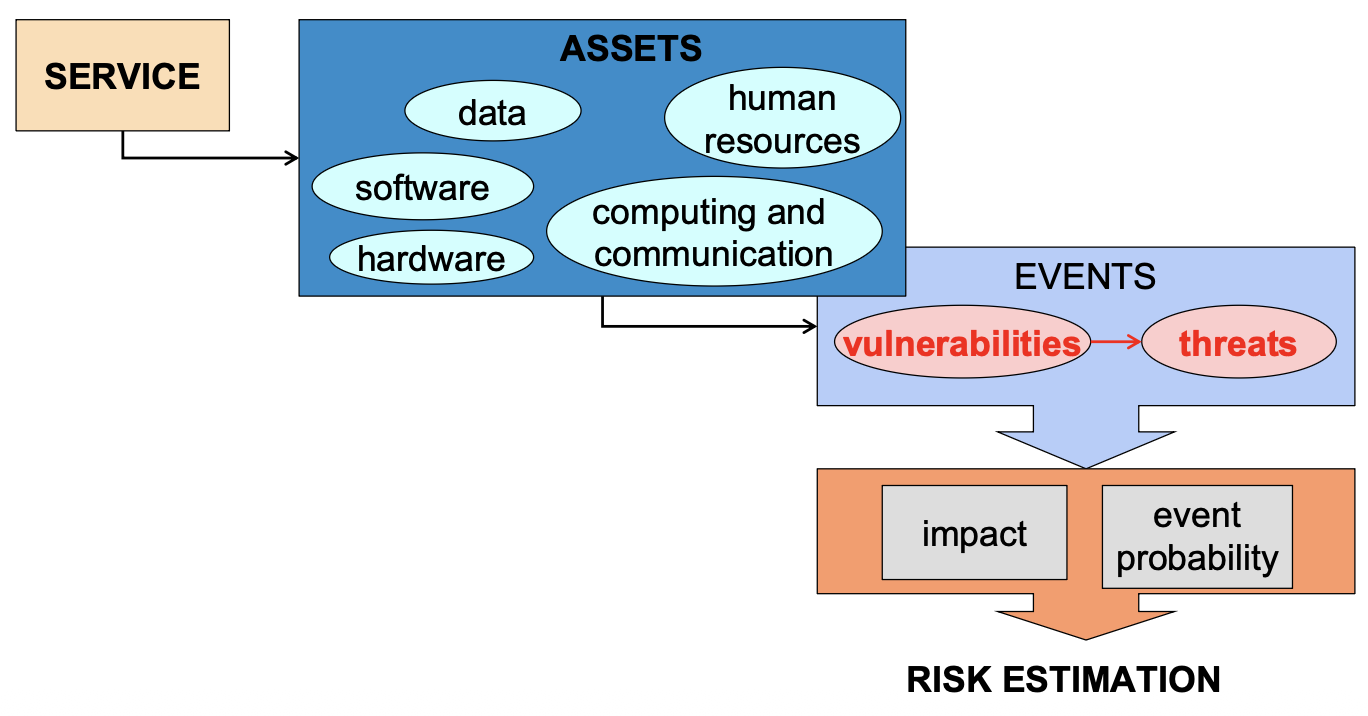
\includegraphics[width=\linewidth]{res/png/estimation.png}
    \caption{}
    \label{}
\end{figure}

Definitions in risk management:
\begin{itemize}
    \item \textbf{Asset}: the set of resources needed for an IT service, such as hardware, software, data, people, and location.

    \item \textbf{Vulnerability}: weakness (in design, implementation, configuration, management) that could be exploited by a \textbf{threat source}. The threat source can be:
    \begin{itemize}
        \item Adversarial (individuals, groups, organizations, or entities).
        \item Non-adversarial (natural disasters, erroneous actions taken by individuals).
    \end{itemize}

    \item \textbf{Threat}: possible deliberate action or accidental event that can cause \textbf{harm to assets} by exploiting a \textbf{vulnerability}.

    \item \textbf{Attack}: threat occurrence (\textbf{deliberate} action). When a threat is realized intentionally, we call it \textbf{security attack}.

    \item \textbf{Negative event}: threat occurrence (accidental event).
\end{itemize}
For more definitions: \url{Source: NIST(2017), An Introduction of Information Security: https://csrc.nist.gov/pubs/sp/800/12/r1/final}

In the end, a company will have many different risks identified, and it needs to prioritize them, keeping into account not only the impact and likelihood, but also the available time and budget. This helps addressing the most important risks first, or maximize the number of risks covered.

To help in evaluating the importance of risks, companies can make a \textbf{risk assessment matrix}, also called risk risk rating matrix or risk heat map:

\begin{figure}[!ht]
    \centering
    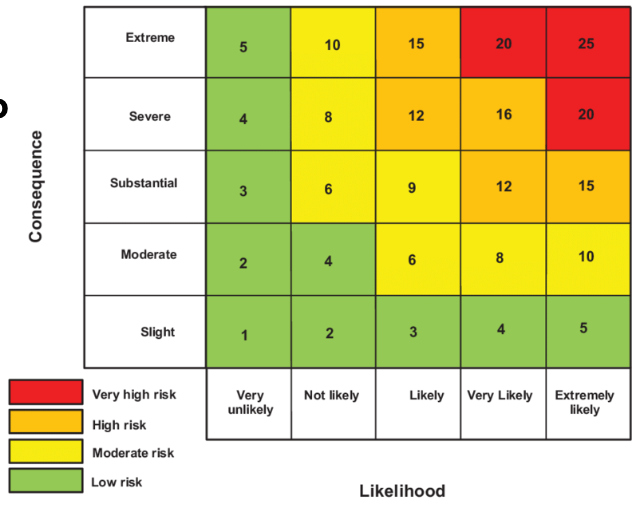
\includegraphics[width=0.5\linewidth]{res/png/ratingMatrix.png}
    \caption{}
    \label{}
\end{figure}

This matrix works by computing a risk index:
\[\text{RiskIndex} = \text{Impact} \times \text{Probability}\]

The risk index summarizes risk using
numbers or categories such as words,
letters, or colors. It allows us to \textbf{prioritize} risks, understand which ones are the most important and how they change over time, compare different risks, and support decision-making. Impact/consequence and probability are commonly assessed on a scale of 1 (minimum) to 5.

\paragraph{Risk management}
Risk management is a fundamental process in every organization because companies and organizations are increasingly exposed to risks related to cybersecurity.

The objective of the risk management process is to \textbf{quantify} the risk, through a repeatable and precise process. The process can start by answering these questions:
\begin{itemize}
    \item What assets do you want to protect?
    \item Why do you want to protect it?
    \item What is its value?
    \item What are the threats? What are the risks?
    \item What are the consequences of its loss?
    \item What will the loss of the information or system cost?
\end{itemize}
For an effective risk management, the following is needed:
\begin{itemize}
    \item Follow a methodology for risk analysis.
    \item Dedicated and qualified personnel
    \item Awareness (and decisions) of the company management
    \item Awareness (and involvement) of the employees
\end{itemize}

For risk management, NIST has proposed a framework of 4 phases:
\begin{enumerate}
    \item Preparation (frame): identification of the assets.

    \item Risk evaluation (assessment): calculating the risk (for example with a risk matrix).

    \item Identification and implementation of countermeasures (security controls), in the hospital/disk example a possible countermeasure is: buy another disk to make redundant copies.

    \item Continuous update of the analysis (monitoring), because the state of security changes over time. This leads back to the previous 3 phases.
\end{enumerate}

Relations in the risk management field:

\begin{figure}[!ht]
    \centering
    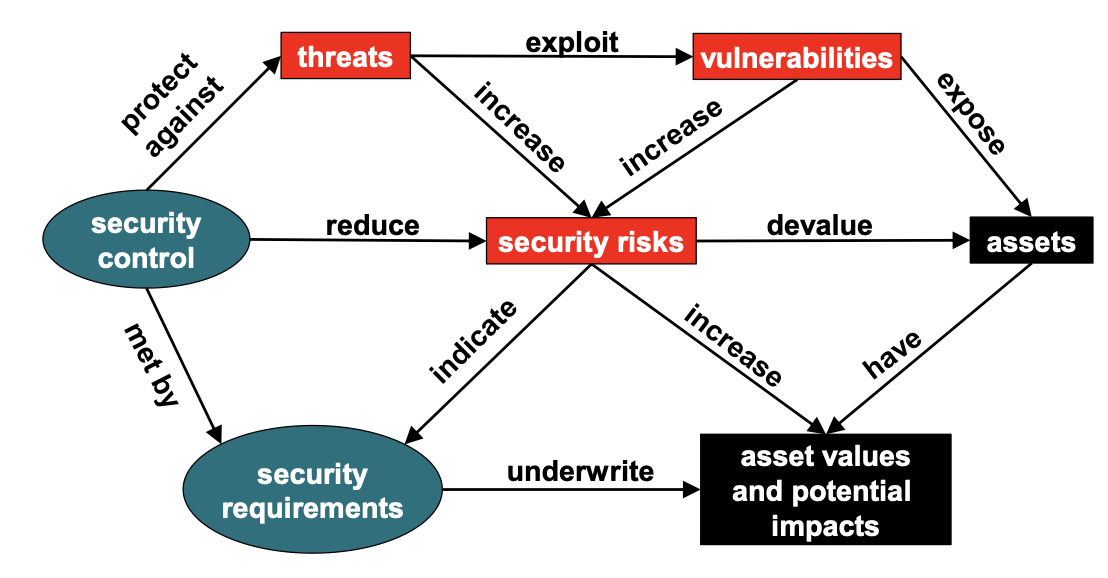
\includegraphics[width=\linewidth]{res/png/riskmanagementfield.png}
    \caption{}
    \label{}
\end{figure}

The \textbf{security plan} is a document that companies use, and it contains the countermeasures adopted to counter the risks:

\begin{figure}[!ht]
    \centering
    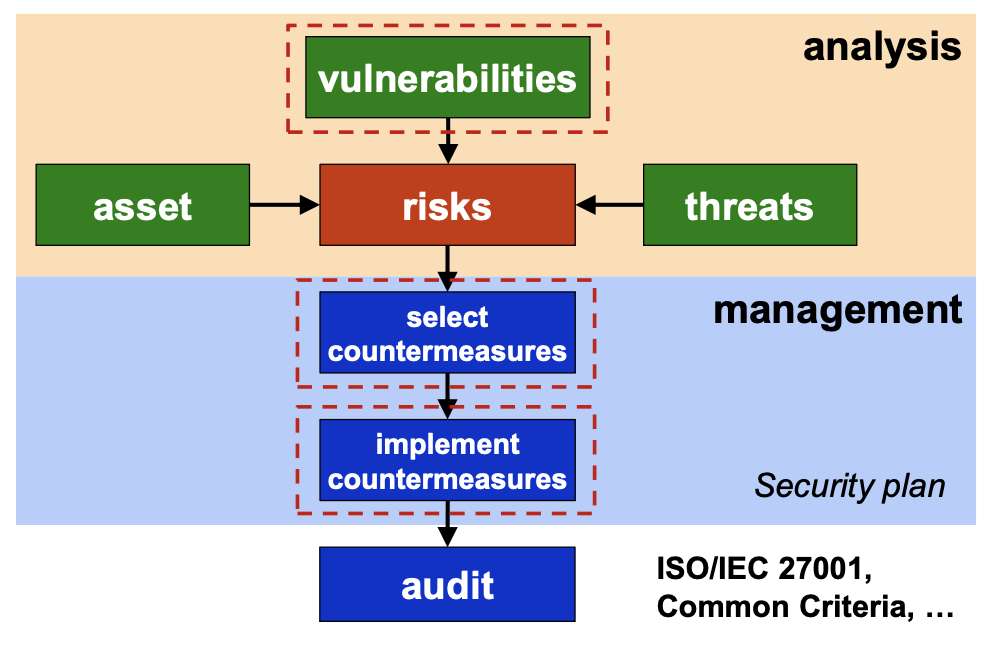
\includegraphics[width=0.5\linewidth]{res/png/securityplan.png}
    \caption{}
    \label{}
\end{figure}

An \textbf{audit} is when someone from an external party comes to evaluate both the security plan and the countermeasures themselves. In companies that have to manage extremely sensitive data (like banks), audit is mandatory and more strict. Typically the auditor uses specific standards, like ISO/IEC 27001, Common Criteria, etc.

\paragraph{High level plan for thinking security}
At a high level, the security of a system/organization is planned in steps:
\begin{itemize}
    \item We need to define a \textbf{security policy}. A security policy defines what you want to achieve from the security point of view.

    \item We need to think of the \textbf{threat model}: model who the attackers are and what resources they have. This implies making some assumptions.

    \item Final goal: no way for the attacker to violate the security policy within the threat model. Threat model is very important: if the threat model is wrong, you may lose security.
\end{itemize}

So, first we define our attacker, and then we define solutions that resist that attacker.

Example: assume we're on vacation and we want to protect our cash money, let's assume we put it in our safe inside our hotel room, and we go outside. The assumption we made is that an attacker can come into our room and is unable to hack the safe. But if the attacker is the manager of the hotel, he/she has the keys of all the safes in the hotel. If we, instead, expect this as our threat model, then a better solution would be to bring the money with us.

Security policies become quite complex: composed of an aggregate of directives, regulations, rules, and practices that prescribes how an organization manages, protects, and distributes information.

As we said, the security policy is a \textbf{vital} component in any company applying information security. It is a requirement of legislation like HIPAA, Sarbanes-Oxley, or regulations and standards like PCI-DSS, ISO 27001, SOC2. Even when not required, it is often a practical necessity to meet stringent security and data privacy requirements.

An \textbf{IT security policy} is a document spelling out the rules, expectations and overall approach that an organization (system) uses to achieve and maintain C.I.A of its data. It answers 'what' and 'why' from the security point of view.

This document is used in conjunction with other types of documentation, e.g. security controls and procedures (which answers ‘how’): specific algorithms, techniques, administrative procedures.

The NIST SP 800-12 defines one possible structured security policy \textbf{format}.

Security policy is important because defining rules is one of the first steps.

\paragraph{Monitoring}
Security analysis and management is an \textbf{iterative} process: design, update threat models and choose countermeasures considering technological trends and attacks evolution. For this reason, audit is also periodic. Over time, technology changes (algorithms, protocols), and so do attacks: they're not static and become more sophisticated over time. Attacks are increasingly structured, with several persons/entities involved:
\begin{itemize}
    \item Highly trained users (hackers..): design and control attacks.
    \item Lowly trained users (crackers, script kiddies): run tools for executing the attacks
\end{itemize}
The first attacks were easy, like the Morris worm: a self-replicating program that sends itself to other computers through the internet. Through time, attacks became more and more complex.

\paragraph{What is a secure system?}
Remember: in general, what we want to achieve is a system capable to guarantee some \textbf{security policies}, assuming a \textbf{threat model}. So, as we said, we must:
\begin{itemize}
    \item consider who are the attackers and what resources they have.
    \item make assumptions (if wrong, the threat model fails and the system may be compromised).
\end{itemize}
But this means that any system will never have \textbf{perfect security}: it's difficult to think of all possible ways the attacker might break in, so each system will likely have some breaking point(s) leading to compromise.

Supporting this last point, here's a revised definition of security by Bruce Schneier:
\begin{quote}
If we've learned anything from the past couple of years, it’s that computer security flaws are inevitable. Systems break, vulnerabilities are reported in the press, and still many people put their faith in the next product, or the next upgrade, or the next patch. “This time it’s secure,” they say. So far, it hasn’t been. Security is a process, not a product. Products provide some protection, but the only way to effectively do business in an insecure world is to put processes in place that recognize the inherent insecurity in the products. The trick  is to reduce your risk of exposure
regardless of the products or patches.
\end{quote}

Some security principles:
\begin{itemize}
    \item simplicity
    \item open design
    \item separation of privilege
    \item least privilege
    \item defense in depth
    \item consider human factors
    \item know your threat model
    \item security by design
\end{itemize}
We will discuss only some of them: simplicity, defense in depth, and thread model.

\paragraph{Simplicity}
We should keep designs (in hardware and software) as simple and small as possible, eliminating unnecessary complexity! Simple designs are easy to test and verify thoroughly, and require less maintenance.

The more complex the design, the more likely it is to posses exploitable flaws (vulnerabilities): attackers can find attack paths increasingly ingenious and unforeseen by the defenders. But (perhaps) simplicity is the most difficult principle to honor due to constant demand for new features (hardware and software).

The KISS (Keep It Simple, Stupid) rule must be respected, coined by an aircraft engineer (K. Johnson) at U.S. Navy (in 1960) handing a team of design engineers with the challenge that the jet aircraft they were designing must be repairable by an average mechanic in the field under combat conditions (in order to be competitive, software companies are somewhat under combat conditions..)

In security, software/hardware complexity leaves (a lot of) space to threats.

\textbf{First axiom of engineering}: The more complex a system is, the more difficult will be to check its correctness (implementation, management, operation).

What should security designers do?
\begin{itemize}
    \item \textbf{Reduce the number of components used}, retain only those that are essential.

    \item \textbf{Minimize functionality}, favor minimal installs and disable unused functionality.

    \item \textbf{Minimize the number of interfaces}, simplify their design.
\end{itemize}

Antoine de Saint-Exupéry:
\begin{quote}
Perfection is achieved, not when there is nothing more to add, but when there is nothing left to take away.
\end{quote}

C.N. Parkinson's Third Law:
\begin{quote}
Expansion means complexity and complexity, decay; or to put it even more plainly—the more complex, the sooner dead.
\end{quote}

\paragraph{Know your threat model}
As we said, the threat model is a model of who your attacker is and what resources they have. One of the best ways to counter an attacker is to understand their \textbf{motivations}: if something is valuable, sooner or later someone will try to attack it.

The cyber threats schema is composed of:
\begin{itemize}
    \item \textbf{threat actors} (and their motivations)
    \item \textbf{vulnerable targets} (value for owner and attacker)
    \item \textbf{attack vectors} (vulnerabilities and context): the ways in which the attackers perform the attack.
\end{itemize}

Nowadays, we have many actors and motivations, we can classify them:
\begin{itemize}
    \item \textbf{Cybercriminals}: single individuals or organized groups, seeking financial gain (direct/indirect), often steal data and demand ransom.

    \item Hackers-for-hire: they sell services to people who do not have the skills, e.g. RaaS - ransomware as a service.

    \item APTs (Advanced Persistent threats): nation-state, huge resources, stealthy, see NSA Tailored Access Operations - \url{https://www.schneier.com/blog/archives/2013/12/more_about_the.html}

    \item Hacktivists: politically, socially, or ideologically motivated. They target victims for publicity, to express protests, or promote a cause.

    \item Digital soldiers, terrorists, etc., they target critical infrastructures or data, e.g. power grids, data centers.

    \item Script kiddies: fun, curiosity, pride, looking for reputation.
\end{itemize}

We can also do a classification of motivations:
\begin{itemize}
    \item Financial (main motivation): monetary gains, theft of resources. Examples: credit card stealing, ransomware.

    \item Espionage, political: industrial or military espionage, for political reasons / information warfare. Resources: almost unlimited.

    \item commercial: a kind of business intelligence, aimed to gain business advantage, or to cause direct or indirect loss.

    \item social: political or social agenda, social hacktivism. Resources: institutional groups, independent groups (sometimes highly supported).

    \item individual: disgruntled employees, curiosity, intellectual challenge, vandals. Resources: scarce.

    \item unknown (!): no clear conclusions on their motivations
\end{itemize}

\paragraph{Defense in depth}
It's not enough to have just 1 defense: multiple types of defenses should be layered together. An attacker should have to breach \textbf{all} defenses to successfully attack a system.

However, consider that:
\begin{itemize}
    \item Defenses are not free (security has a cost).

    \item Defenses are often \textbf{less} than the sum of their parts, for example if you buy the same type of firewall, an attacker who managed to compromise (the first) one, he/she will (most probably) be able to compromise also the second one in short time. So, if we have different defenses, they should be as orthogonal as possible.
\end{itemize}
The firewall is a wall between the server and the attackers.

The multiple layers approach is very common in data centers: they need to protect the stored data, so they employ different defense lines, both physically and logically.

The idea of multiple defense lines was, of course, used also in the past: Forte di Exilles (Italy), Walls of Theodosius II in Constantinople (Istanbul, Turkey), and so on.

\section{Security properties}
We said that we need to protect the data in the presence of an attacker, and in order to do that we need to enforce some security properties. Over time, some security properties were defined:

\begin{figure}[!ht]
    \centering
    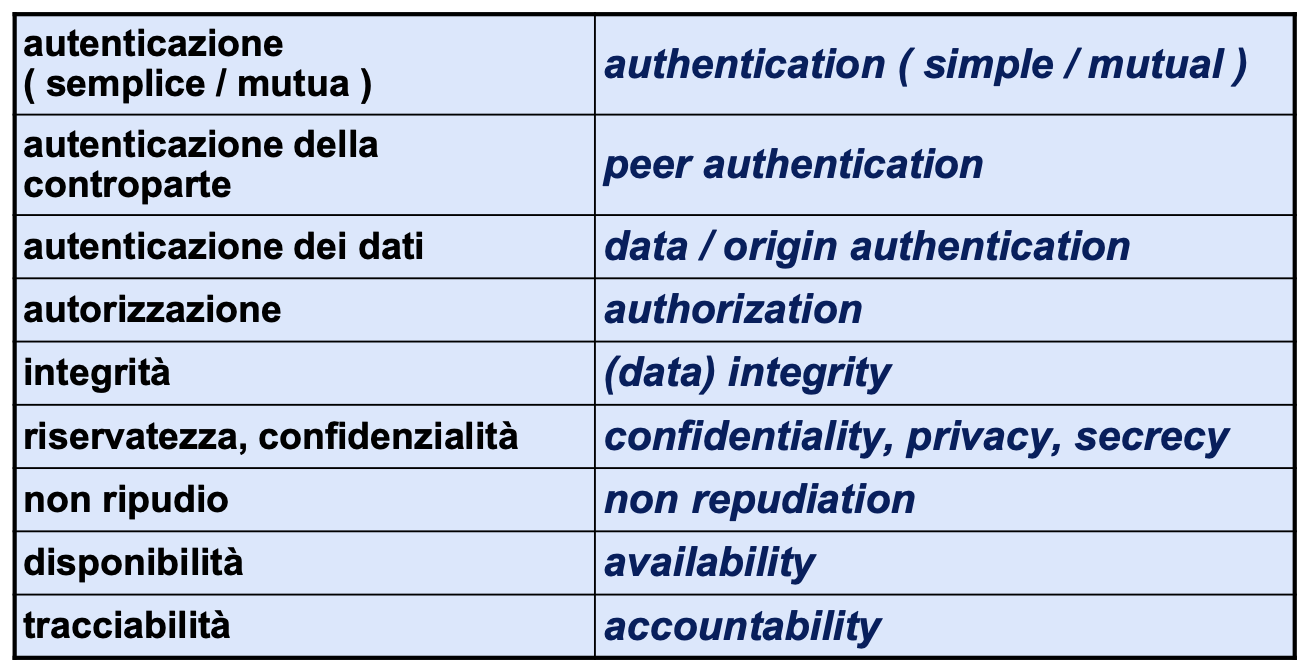
\includegraphics[width=0.5\linewidth]{res/png/secureproperties.png}
    \caption{}
    \label{}
\end{figure}

One of the most important ones, and surely one that came before others, is \textbf{confidentiality}: rendering the data unintelligible to other people who are not allowed to read the data. In fact, cryptography is not new at all, it existed also since Romans.

Another important security property was \textbf{availability}; it became evident over time that an attacker could knock down the availability of important services.

Note that \textbf{not all those properties} are needed in every system, we need to implement only those we require, since they're costly (it depends on the application).

For example, a lot of services, like banks and other public services, want extremely high availability.

Another important property is \textbf{peer authentication}: establishing the authentication of the other part of the communication. Authentication can be single or mutual, we'll see it.

\paragraph{Confidentiality and privacy}
Confidentiality: information is available to read only to authorized parties. Example: Alice sends a message to Bob, only Alice and Bob can understand the content of the message.

Linked to the concept of confidentiality there's the concept of \textbf{privacy}.

Privacy: individuals may control or influence what \textbf{personal} data related to them may be collected and stored and by whom and to whom that information may be disclosed.

\paragraph{Peer authentication}
Entity (peer) authentication: allows to verify that the (communicating) entity is who it says it is. It's used in connection-oriented communication to provide assurance on the identity of the entities connected, and it typically involves some credentials (like username and password).
\begin{itemize}
    \item \textbf{Single authentication}: only one entity authenticates the peer. Example: Alice tries to obtain access to her bank account: the bank performs peer authentication operation to ensure that’s really Alice asking for the information.

    \item \textbf{Mutual authentication}: both entities authenticate to each other.
\end{itemize}
Example where mutual authentication is needed:

\begin{figure}[!ht]
    \centering
    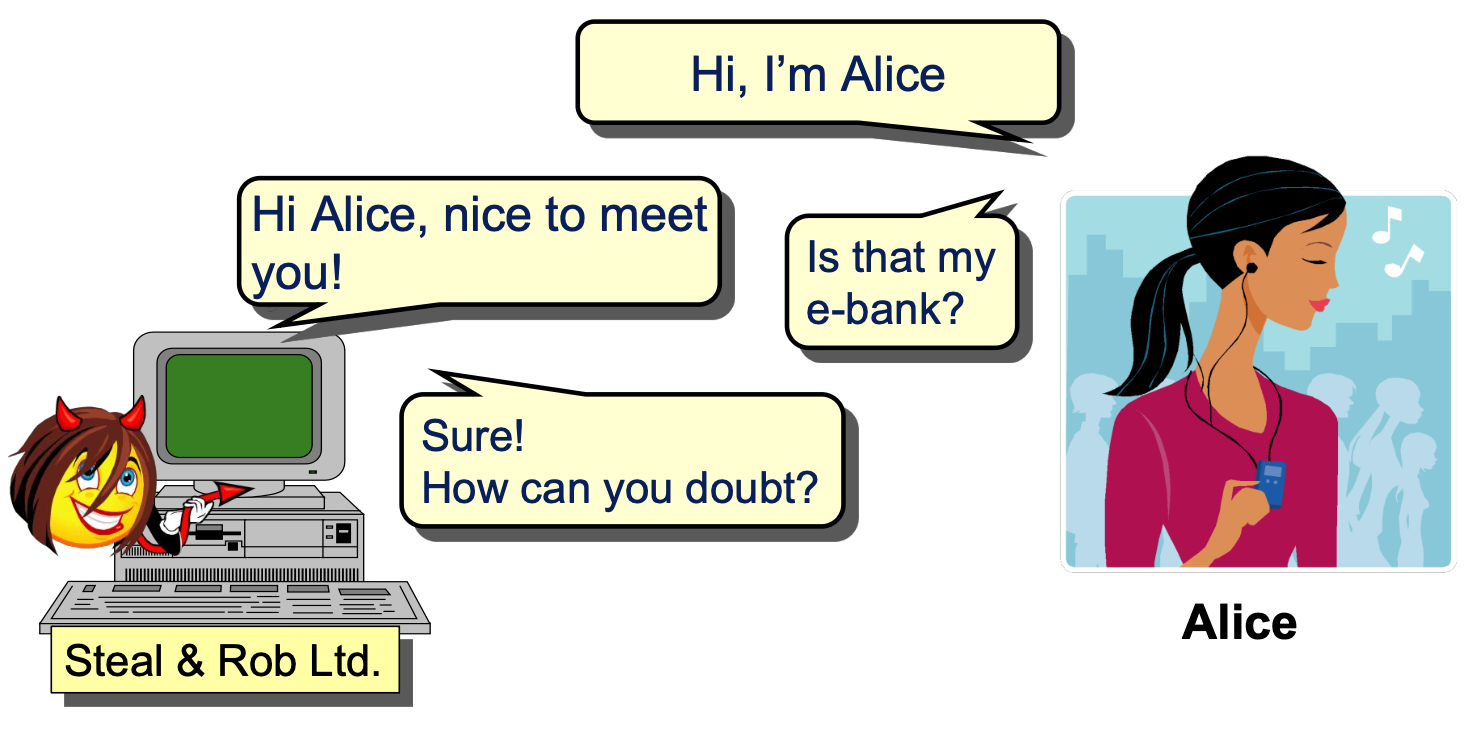
\includegraphics[width=0.5\linewidth]{res/png/mutualauth.png}
    \caption{}
    \label{}
\end{figure}

\paragraph{Data/origin authentication}
Data/Origin authentication allows to verify that the data is coming from an asserted party. It is needed when we have communications \textbf{without connections} (like email, which is a \textbf{connectionless} system). It's achieved by \textbf{attaching something to the message} that allows the receiver to verify that the message comes from the right source. Also, if we have a channel, it's not sufficient to perform peer authentication at the beginning, because an attacker could insert himself in the communication after it has been established. So, we also need data authentication together with peer authentication.

\paragraph{Integrity}
(Data) Integrity allows to detect if data was \textbf{modified}:

\begin{figure}[!ht]
    \centering
    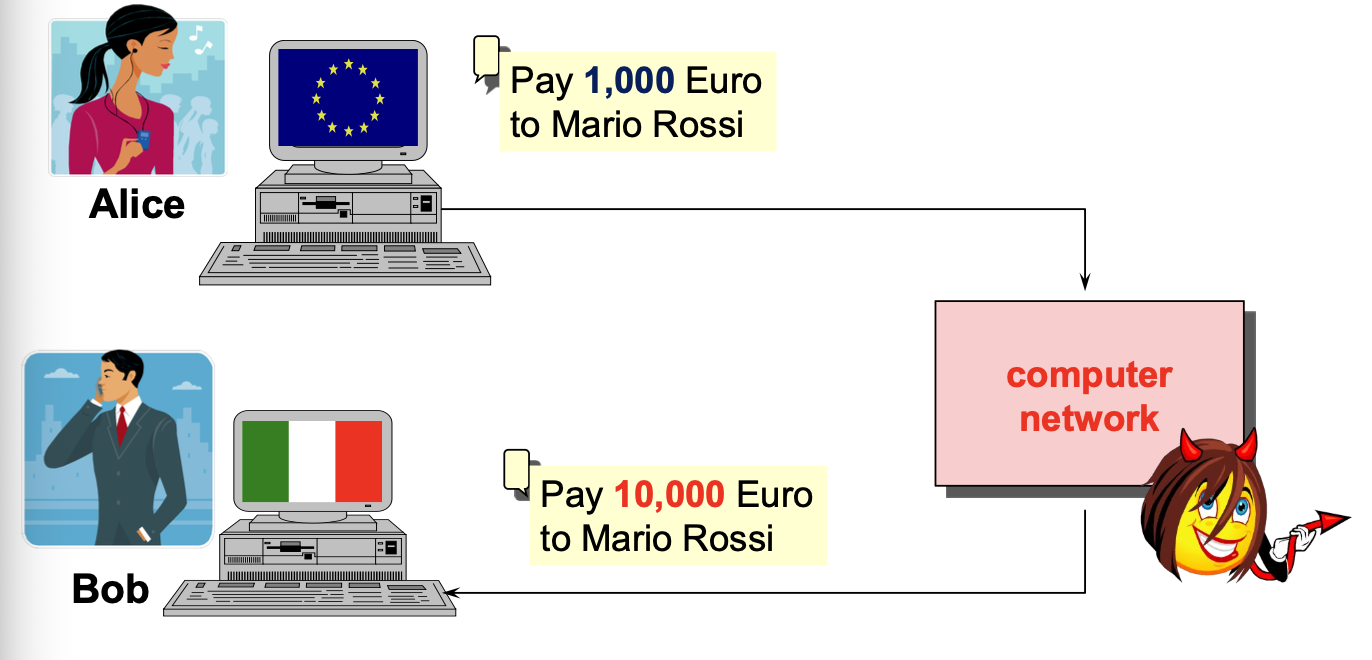
\includegraphics[width=0.5\linewidth]{res/png/integrity.png}
    \caption{}
    \label{}
\end{figure}

In the example, Alice sends a message to Bob. Eve intercepts the message and
modifies it. Data integrity allows Bob to detect whether the message was
modified (replayed, filtered) on its way.

Data integrity needs to happen not only when the data is traveling, but also for \textbf{stored} data. Typically we'll attach something to the data to verify integrity.

Another potential integrity attack is not about modifying, but rather \textbf{data cancellation/filtering}: the attacker can delete the message altogether or filter it. If our system implements the integrity property, the receiver can detect wether the message was filtered on its way.

Another integrity aspect is the \textbf{data replay}: sending the same message multiple times. Not to be confused with a \textbf{relay} attack: one where the attacker intercepts the data and sends it to another attacker.

\begin{figure}[!ht]
    \centering
    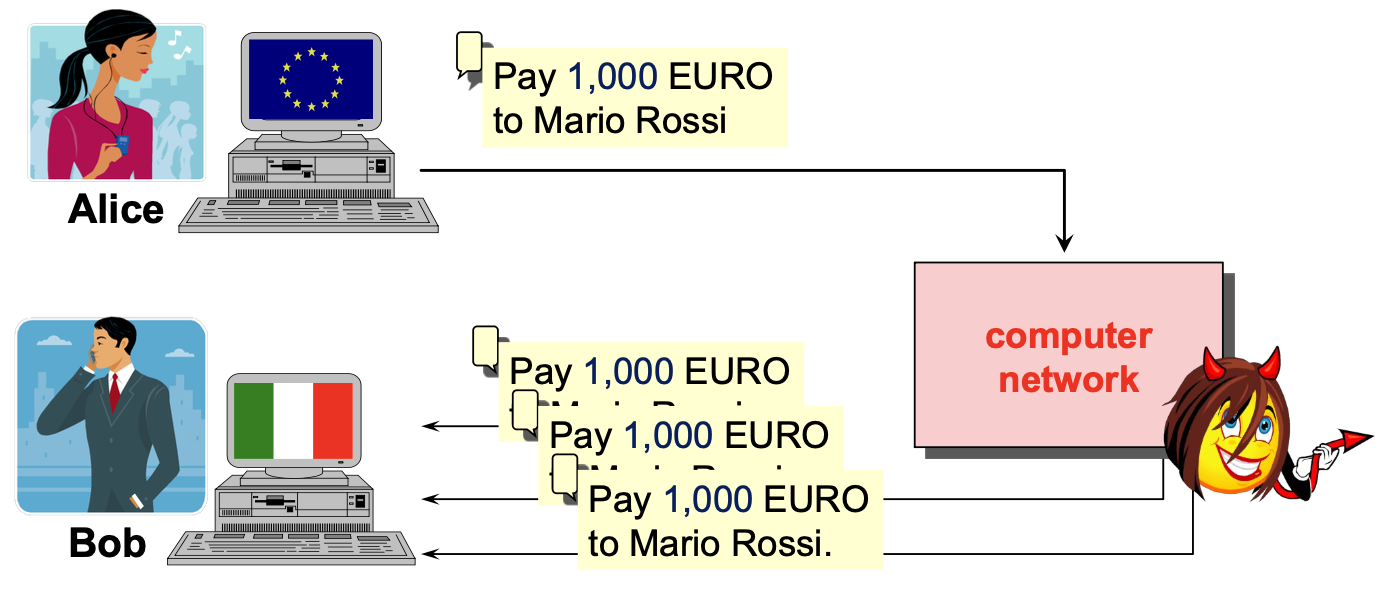
\includegraphics[width=0.5\linewidth]{res/png/3reply3.png}
    \caption{}
    \label{}
\end{figure}

Data integrity allows for Bob to detect that the message was replayed, on its way, we can implement this by numbering messages.

\paragraph{Authorization (access control)}
Access control/Authorization: guarantees that only authorized parties can use or access specific resources. Example: Alice wants to use Barbara’s car, she must be authorized to get that car.

\paragraph{Non repudiation, availability, accountability}
\textbf{Availability}: assures that authorized entities have access to resources (services, data) when they need them. Example: a web site should continue to provide its service(s) even though the server is in under attack (like a denial of service attack): this is done if we provide the same service through different servers, so if one of them is attacked, the other servers can still provide the service without loss of availability.

\textbf{Accountability}: allows to keep track of who does what and when. Typically achieved through logs. Typically very important for investigations.

\textbf{Non-repudiation} is a bit more complex. It guarantees that an entity cannot deny that it has performed an action. It creates a formal proof - acceptable by a court of justice - that gives undeniable evidence of the data creator (very strong property).

Example: Alice sends Bob a signed contract. Non-repudiation ensures that Alice \textbf{can not claim} that the signature was produced by somebody else.

There are several facets to this property: sender authentication / identification, integrity, and so on, in fact: non-repudiation is \textbf{stronger} than just authentication. It's normally associated not only to technical aspects but also to specific procedures performed voluntarily; for this reason it's \textbf{not} achieved simply with protocols or procedures that perform automatic actions on the user’s behalf, since automatic procedures lack the \textbf{voluntary} aspect. For example, an automatic signature produced by a system can't be accepted; a manually written signature can be.

For example: \textbf{authentication is not identification}. Authentication can provide some weak evidence that Alice is really Alice, for example with a password. But maybe someone else typed Alice's password instead of her. To demonstrate that it was really Alice, nowadays we often use biometric systems, like fingerprints or eye imprints.

\paragraph{Data protection}
As we already said, each security property considers always the three cases of data protection:
\begin{itemize}
    \item data in transit: data transmitted over a communication channel.
    \item data at rest: data stored in a memory device.
    \item data at work: data in RAM for use by a process.
\end{itemize}

\section{Technological and non-
technological security attacks}
Let's see some basic technological problems. Before continuing, let's remember that an IP address identifies a node in a network (layer 3), while MAC address identifies a device in layer 2.

First of all, networks are still insecure:
\begin{itemize}
    \item Some traffic is (still) in clear e.g., network management protocols (DHCP, ARP), widely used nowadays. Anybody that sniffs the communication could read and modify messages.

    \item LANs operate in broadcast: anytime anyone sends a message in a LAN, the message arrives to everyone else connected: anyone could intercept it, replay it, modify it, inject a new message, etc.

    \item Geographical connections are NOT made through end-to-end dedicated lines anymore (as in the centralized model, unicast) but through shared lines and third-party routers. So there are a lot of messages passing through many different nodes and devices. So it's easier to attack the communication.

    \item Data (associations) can get cached – for efficiency:
    \begin{itemize}
        \item (IP address, MAC address) in the ARP protocol.
        \item (IP address, name) in the DNS protocol.
    \end{itemize}
    These associations can be manipulated to perform attacks, as we'll see with the ARP poisoning attacks.
\end{itemize}

Then, authentication can be problematic:
\begin{itemize}
    \item (weak) user authentication (password-based)
    \item server authentication: it's unfortunately not done in some protocols (e.g. DNS, ARP, DHCP, and others).
\end{itemize}

Finally, software contains bugs (vulnerabilities), an \textbf{malware} exists.

\paragraph{Some classes of attacks}
\begin{itemize}
    \item \textbf{IP spoofing / shadow server}: someone uses the address of another host, to take its place as a client (and hide its own actions) or as a server. So the attacker modifies the source IP address.

    \item \textbf{Packet sniffing}: the content of the network packets (e.g. passwords and/or sensitive data) are read by unauthorized parties.

    \item \textbf{Connection hijacking / data spoofing}: data inserted / modified / canceled during transmission.

    \item \textbf{Denial of service (DoS) and distributed DoS (DDoS)}: the functionality of a service is limited or disrupted (e.g. ping bombing).
\end{itemize}
Let's analyze them one by one.

\paragraph{Packet sniffing (eavesdropping)}

\begin{figure}[!ht]
    \centering
    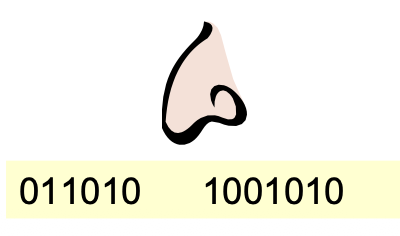
\includegraphics[width=0.5\linewidth]{res/png/PacketSniffing.png}
    \caption{}
    \label{}
\end{figure}

It's a \textbf{passive} attack, reading the packets addressed to another network node, nowadays performed with a traffic sniffer.

It's easy to do in broadcast networks (e.g. LAN) or at the switching nodes (e.g. router, switch): in laboratory 1 we'll use some tools to perform sniffing in the LAN: in a LAN we can put net card in promiscuous mode to intercept \textbf{all} traffic directed to the LAN.

On switching nodes (like routers): there is a specific port, the \textbf{mirror port}, that can be used for diagnostic; if we read this port we can perform packet sniffing by reading all the traffic.

\begin{itemize}
    \item Attacks allow to intercept anything (password, data, other data)

    \item Through \textbf{traffic analysis}, attackers can determine location, identity of peers, frequency/length of messages, even if data is encrypted.
\end{itemize}
Then the question is: how can we defend from an attacker's traffic analysis? An answer could be: send data \textbf{all the time}, without stopping. Most of the data sent this way is \textbf{meaningless}, it simply serves the function of avoiding the traffic analysis.

\paragraph{IP spoofing}
IP Spoofing is an \textbf{active attack}, where the attacker forges the source network address: typically the IP address is forged, but it's equally easy to forge link layer address (MAC address, and so on). For this reason, a better name would be \textbf{source address spoofing}, not just IP.

The attacker creates IP packets which have a modified source address in order to either hide the identity of the sender, to impersonate another computer system, or both: the attacker puts the IP of someone else to make others believe the message comes from that person.

Possible attacks exploiting IP spoofing:
\begin{itemize}
    \item DDoS: attacker wants to hide his real IP address.

    \item Data forging (e.g. fake email): attacker creates data and wants to make appear as coming from a legitimate user.

    \item (unauthorized) Access to systems: attacker wants to get access to systems providing access based on IP address. Specific to ‘r’ commands, e.g. \texttt{rlogin}. Actually, nowadays this system is not used anymore, the IP address is not enough to access systems anymore.

    \item DNS shadow server.

    \item Amplification DoS (with DNS or the time server).

    \item Ping bombing hiding his real IP address.
\end{itemize}

\paragraph{Denial of Service (DoS)}
DoS is an \textbf{active attack} that keeps a host busy or exhausts its resources, so that the host can't provide its services. For example the mail space can be exhausted, so that no more mails can be received. Or an attacker can saturate the Log files on a destination, because in the log files it's tracked \textbf{who did what} (typically the first thing the attackers do is to saturate the log files, and then they do the attack).

Examples:
\begin{itemize}
    \item mail / log saturation.
    \item ping flooding (“ping bombing”). \texttt{ping} is a command that exploits the ICMP protocol, widely used in networking to see if another node is alive. But an attacker can bombard a node with pings, keeping it forever busy responding to pings.
    \item TCP SYN attack, we'll see later during the course.
    \item DNS floods.
\end{itemize}
So, attackers block the use of a system/device. There are no real countermeasures: we can monitor and oversize (i.e. have a bigger disk) but they're not real solutions, because the attacker can just send more data to fill even the bigger disk.

\paragraph{Distributed Denial of Service (DDoS)}
This is a variant of the DoS. A DDoS attack multiplies the effect of a DoS attack by exploiting many compromised nodes (daemons). Steps:
\begin{enumerate}
    \item The attacker individuates the \textbf{victim}.

    \item The attacker exploits vulnerabilities in multiple remote nodes to install a malware (a software that performs malicious operations), with auto-update feature. These nodes become \textbf{zombies} (or daemons, part of a Botnet) that might NOT know that are exploited for an attack, for example a PC somewhere that's not getting upgraded in years.

    \item The attacker chooses some zombies as \textbf{masters}, whose role is to synchronize the zombies during the attack (typically controlled over encrypted channels).

    \item The attacker communicates to the master(s) to launch the attack and he/she disconnects from the network (masters operate autonomously).

    \item At a specific time, the master(s) communicate to the zombies to launch the attack, simultaneously, against a victim.
\end{enumerate}

\begin{figure}[!ht]
    \centering
    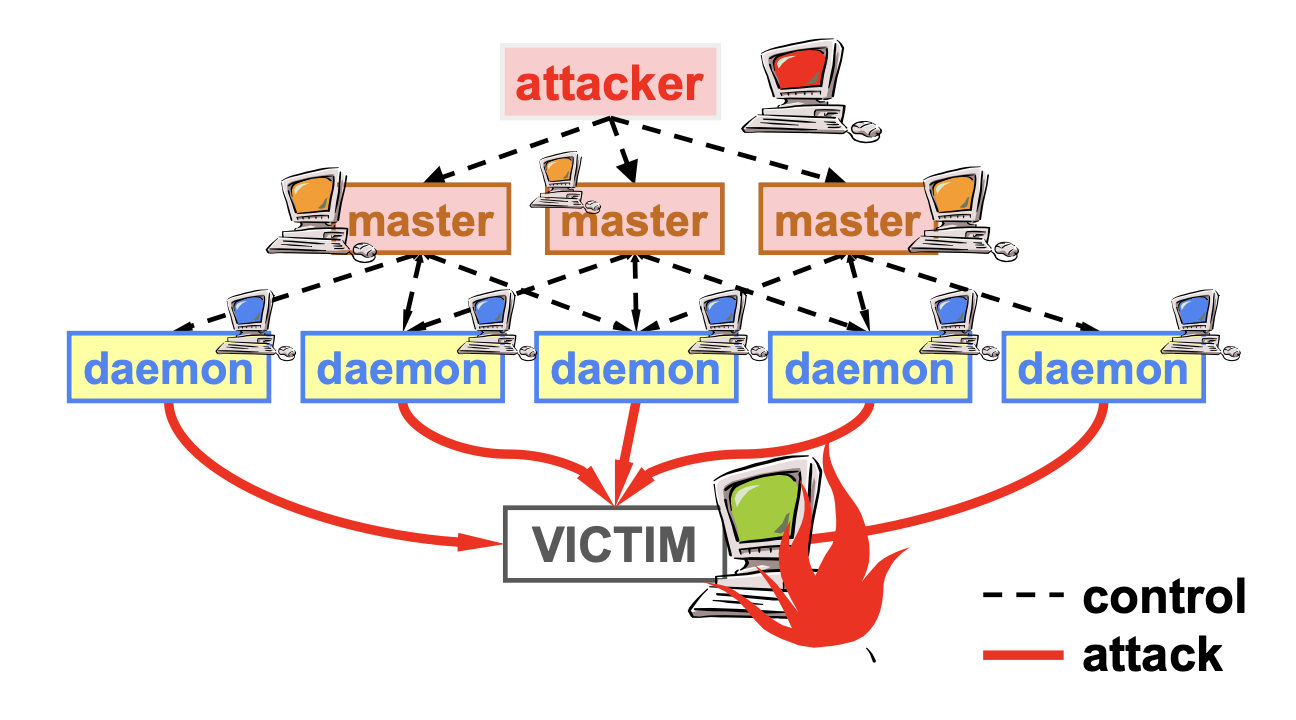
\includegraphics[width=0.5\linewidth]{res/png/DDos.png}
    \caption{}
    \label{}
\end{figure}

\paragraph{Reflective DDoS}
Also known as Amplification DDoS attacks. Reflective DDoS are Attacks facilitated by adversaries exploiting publicly used Internet Application Services, such as the Domain Name System (DNS, it resolves names to IP addresses in internet) or Network Time Protocol (NTP, it distributes \textbf{time} in internet) public servers. Amplification DDoS attacks occur either through DNS Amplification attacks or through the NTP Service. By spoofing the source IP address of these services, attackers can amplify traffic and disguise their identity at the same time.

To explain further: these protocols have a particularity. First of all, they must be always available, because they provide useful and fundamental services to the internet, they can't be turned off. NTP has the particularity that 1 byte is sent and  for example 70 bytes can be received back (in other words, there's an \textbf{amplification}). Also DNS has an \textbf{amplification factor}: the size of the response is much greater than the size of the request.

Typical DNS amplification is 70:1, but NTP amplification can be 20-200:1.

We can imagine a bot with multiple zombies that contribute to the attack; these zombies will send requests to a DNS or NTP server, that has to run all the time. When the zombies send this request, they use a \textbf{spoofed} IP address, the IP address of the victim:

\begin{figure}[!ht]
    \centering
    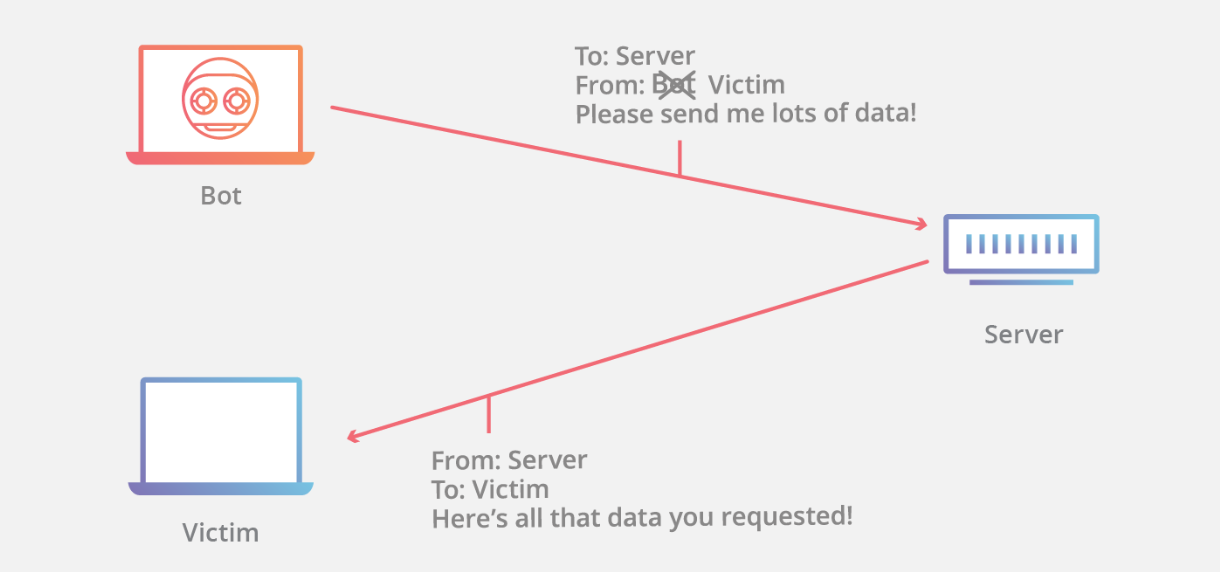
\includegraphics[width=0.5\linewidth]{res/png/reflectiveDDos.png}
    \caption{}
    \label{}
\end{figure}

Of course, the server responds to the request by sending data to the victim, since that's how the protocol works:

\begin{figure}[!ht]
    \centering
    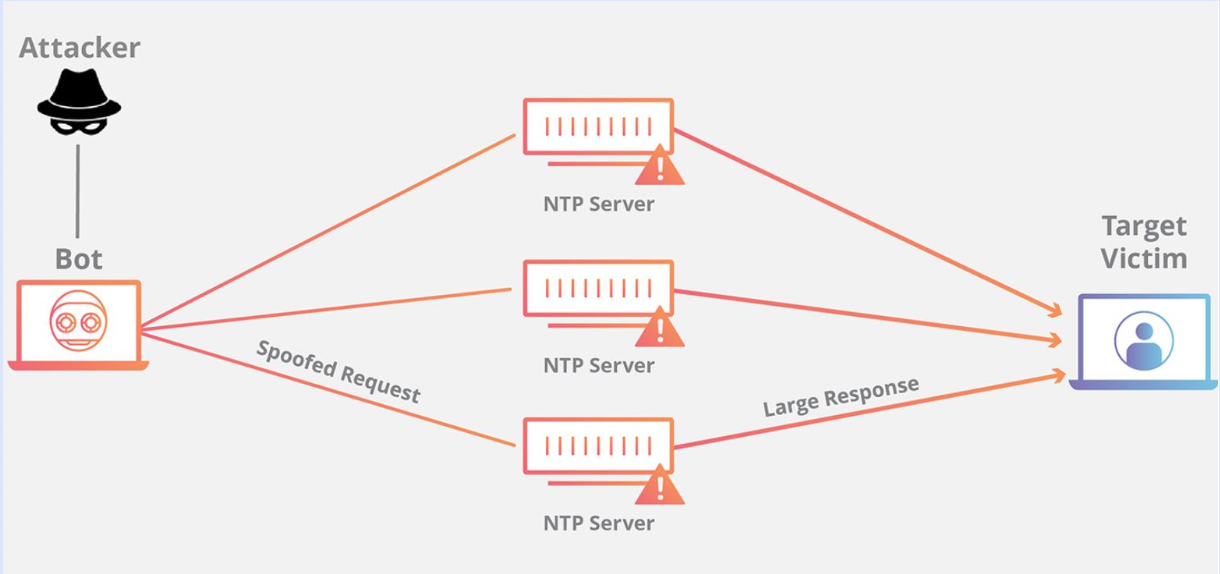
\includegraphics[width=0.5\linewidth]{res/png/ddosss.png}
    \caption{}
    \label{}
\end{figure}

Note that to send a request from bot to the server we don't even need high bandwidth: even a very small device can work, since the servers can amplify the data sent.

Why can’t server block the requests? if the source IP address is falsified and continuously randomized, blocking malicious requests becomes difficult.

\paragraph{DNS}
Small review of how DNS works: a user sends a request to a DNS server to find out the IP address of a website the user wants to visit. So, the request contains the website's hostname (for example polito.it), and the DNS server answers with the corresponding IP address.

The client:
\begin{itemize}
    \item checks its network settings to find a local DNS server
    \item sends a DNS request (UDP, port 53)
    \item if a record (Resource Record, RR) is found in the DNS server, it answers with a DNS reply
    \item If the NS does not have a record for this hostname, the local NS contacts recursively or iteratively other NSs. Finally, it caches the DNS response.
\end{itemize}
For example, if a client in Italy wants to connect with a Japanese website, probably it's not in the cache of the local NS, so the local NS will contact other NS until it can find the correct IP address.

\paragraph{Shadow server}
The shadow server is a fake server that shows itself to the victims by exploiting DNS. The victim sends a DNS request to a nameserver; the attacker steals the request and replies with a malicious DNS response. Inside the fake response, the attacker can use another IP address, associated with the attacker, so the victim will end up connected not with the original service he desired, but with an host related to the attacker.

So, the attacker requires packet sniffing, and then spoofing to generate the fake DNS responses.

The client will accept the responses, as they're not authenticated. There is also the possibility of DoS: if the attacker puts the IP address of a host that does not exist, then the victim will connect to this host that doesn't exist, so the service to the victim is denied.

When the request is sent to the local nameserver, it arrives to it, and the nameserver gives back a response to the victim. But, if this answer arrives \textbf{later} than the attacker's answer, the nameserver's response will be discarded as a duplicate! So, the attacker must be \textbf{faster} than the real server, or the attacker must keep the server \textbf{busy} and slow, for example with a DoS.

We can also do a shadow server attack by faking a DHCP server (those we use to connect to a network): the fake DHCP server will return fake network configuration, for example IP address that does not exist (so we can make a DoS as we just said), or the IP of a friend of the attacker, or any other.

Shadow server is of course an \textbf{active} attack: we give bad answer to the victim, in order to steal his data or deny him a service.

\paragraph{ARP protocol}
We use ARP to discover the MAC address of a node when knowing its IP address. An ARP broadcast request is sent, then the response is received, and the MAC saved in the cache for efficiency reason (to contact again that host).

\paragraph{ARP Poisoning}
An attacker can do for example \textbf{ARP poisoning}: sending to the victim a wrong MAC address (for example the attacker's one). In order to work, the ARP poisoning must be frequent, otherwise the ARP table will cleanse itself.

In the lab, we use \textbf{ettercap} to do this attack

\paragraph{Man in the middle (MITM)}
MITM: an attacker takes control of a communication channel transporting data between 2 parties. It's an \textbf{active attack}. It's also called communication hijacking or data spoofing, and it allows to read, insert, delete, block or manipulate the traffic. All the traffic will flow through the man in the middle. It can be logical or physical.

Countermeasures against MITM: we can apply \textbf{security properties} to the packets that are exchanged between nodes. Example: suppose we're in Turin and we want to send 100 boxes (that correspond to packets) to our friend in Milan. We do something to protect the boxes and the contend inside, for example putting a stamp on the box with destination and origin; we can put a \textbf{seal} on the box to ensure that no one else has opened it; we can \textbf{number} the boxes, so if one is missing we can understand there was a problem.

The same exact methods can be applied to packets, so who receives the packets can check that they come from the sender, they've not been modified, they've not been lost, and so on.

Numbering packets is called \textbf{serialization}.

Variation of MITM: MATE (Man at the End). This is an attacker running just on an endpoint: not in the middle, but at the end of a communication. This can be done by installing a software (e.g. a keylogger, malware, browser extension) in a host.

\section{Software vulnerabilities, malware}
A class of attacks that nowadays are very serious. Today, software is affected by many vulnerabilities, that can be exploited to perform the attacks.

\paragraph{CVE (Common Vulnerabilities and Exposures)}
NIST proposed to create and maintain a DB that contains information on all the software/firmware/code that could contain vulnerabilities. Not only applications (installed software), but file and services on the HD, or even just mobile code, ode in memory, firmware (e.g. the BIOS).

They are indexed in the DB: they have a number. There are more than 200.000 CVEs. They also have an indication on how serious they are, the CVSS score.

Companies check periodically if the software they're using is on the CVEs. If it is, they must quickly patch the software. Of course, it's a continuous process.

Network scanning is very important: for the attacker to find potential attacks, and for the defenders to periodically find vulnerabilities (\textbf{vulnerabilities assessment}). In each organization there's people that periodically perform scannings to check all interfaces of the system, looking for vulnerabilities. This process is usually structured, and there are some tools that can be used to perform it. For example Nexus (old tool for vulnerability scanning).

\paragraph{Window of exposure}
Let's see the process to handle the vulnerabilities. Imagine we're running a software from a famous vendor (e.g. Microsoft). Then, at a certain point, a vulnerability on that software is discovered. But vulnerability found isn't immediately a problem, because the attackers must first write the exploit. Then, the exploit is made public. Between this moment (exploit has been made public) and the moment the security patch goes live, there is a \textbf{window of exposure} during which the risk of being attacked is high. In other words, it's a period where we're informed of a vulnerability but there's no solution.

During the window of exposure we can adopt some precautions: we can notify our vendors and our customers about the problem. We can turn off (deactivate) some of our services, or completely deactivate some server / node. We could even monitor with more attention some areas of our network, for example if we see some area with abnormally low traffic, it could mean that area has been already attacked.

The moment the vulnerability is discovered, it's called zero-day, because they have 0 days to be solved. They are the most dangerous vulnerabilities today, because as soon as it's discovered, there's still no solution yet, but the vulnerability can still do a ton of damage quickly in the 0-day.

After, the first patch gets been written and published. In the CVEs DB there's usually the patch link also, so people can download the patch if they're under that attack.

But, not everyone installs the patch immediately. Also, vendors don't release all patches immediately, but rather on a structured basis (depending on the vendors), and not all the clients install the patched all at the same time, depending on the client.

So, after the moment of discovery of a patch, some time passes until the patch is widely known and then finally installed. Before the patch is actually installed, \textbf{attackers can and will} attack victims.

\paragraph{Virus and Worm (malware)}
A \textbf{virus} is a program that, if run by the user, can provoke damage to the system. It embeds itself into a host program or file that contains some form of executable content. It's propagated by humans (involuntarily), for example from inserting into a device a USB flash drive or clicking on an e-mail attachment. The virus is mainly propagated through humans.

A \textbf{worm} is different from the virus, because it's a program that propagates itself automatically, exploiting network protocols and daemons (without attaching to other programs). They try to spread as much as possible without human interaction, to generate DoS.

Sometimes software are deployed with automatic updates, but if that gets bugged it can result in a vulnerability, because the automatic update works by going to the vendor's website and download the last version of the software, but this downloaded software can contain a virus.

\textbf{Countermeasures} to viruses and worms is awareness, installing patches, and using an antivirus.

\paragraph{Trojan and backdoors}
A \textbf{Trojan} is a software that contains a dangerous payload. It's inside another application that performs good operations, like an editor for example. If the editor is infected with the Trojan, while we edit the file the Trojan is doing other things in the background, for example deleting files or reading our messages.

Trojans are very hidden and act on the background, while we're performing normal operation.

\textbf{Backdoor} attack takes inspiration from the backdoor of houses (the second interface to enter). Backdoor is a way to get access remotely to an application, not by the main entrance.

\paragraph{Rootkit (malware)}
Rootkit is a program that stays hidden. It can be used for:
\begin{itemize}
    \item surveillance: monitor and track what a user is doing
    \item data exfiltration (the theft or unauthorized removal or movement of any data from a device)
    \item perform intrusions on the host.
\end{itemize}
The rootkit modifies data structures and other things that \textbf{don't} impact the normal OS functions, so the OS continues to work normally. In general, the rootkit erases the log files to hide its existence: one of the first things an attacker does it invalidate/erase the logs.

A \textbf{Keylogger} is a software that records the keystrokes of a victim.

\paragraph{Malware food chain}
In the past, malware was created for reputation or curiosity, but now they're just made for \textbf{profit}. Suppose someone discovers vulnerabilities or malicious code. Such a person could \textbf{sell} this knowledge in the dark web (vulnerability marketplace) for a good sum of money. In this place, there are some who sell vulnerabilities and some who buy them: developers of malware who try to develop exploits in order to be the first ones to \textbf{attack} (zero-day vulnerability). The vulnerability gets bought by developers of malware, then they further sell the malware in the malware toolkit market, and then the malware is distributed to victims via malware distributors (spam, web, etc.).

In this food chain, every actor has something to gain, except for the victims.

Then there's the \textbf{bug bounty}: companies put a bounty on any vulnerabilities that can be found: if people find and submit these vulnerabilities to the company, the company will pay them. This \textbf{breaks the food chain}, because now a person seeking profit can instead do this!

\paragraph{Ransomware}
Ransomware is an attack where threat actors take control of a target's assets and demand a ransom in exchange for the return of the asset's availability and confidentiality.

Usually, even if the victim pays, they don't get back all the original data they had, or sometimes they don't get anything. A report in 2021 indicates that 32\% of companies affected by the ransom actually paid, but only 8\% got the whole data back, and 29\% recovered up to half of the data. 65\% is the average amount of data recovered after the payment. But even them, companies have to pay costs for recovery of the system and \textbf{changing} the system to not be affected again.

\paragraph{Base problems (non technological)}
Computer security is not only about computers, but also about people, that have critical roles:
\begin{itemize}
    \item holders of important information
    \item operators and maintainers of security critical infrastructure
    \item users of apps managing sensitive data (credit card numbers, health data, banking details)
\end{itemize}
In many cases, humans are actually the \textbf{weakest} link of security chain, because they have:
\begin{itemize}
    \item low awareness of security problems
    \item tendency to perform errors (especially in conditions of stress, frustration, fatigue, work overloading)
    \item natural tendency to trust
\end{itemize}

\paragraph{Social engineering}
Social engineering is the \textbf{psychological manipulation of people} into performing actions or disclosing confidential information.

Kevin Mitnick wrote "The Art of Deception", a book about social engineering, where he proposed several techniques for social engineering attacks.

Usually, naive users are attacked, especially if they're put under stress. But also experienced users, under stress or other factors, can perform errors. Social engineering attacks are usually successful because they exploit low user awareness, and human emotions and weaknesses (fear, tendency to trust, possibility to gain fortunes, and so on).

In general, a social engineering attacker shows acquaintance with the company's procedures, habits and personnel (e.g. friend of another friend, or maybe he genuinely established a human relationship in the past just to gain the trust).

Social engineering attacks are not only online; they can also be physical attacks: \textbf{baiting} (dropping a USB key with a malware on the floor), or \textbf{tailgating}: wait for an employee to open a door, to also get in.

\paragraph{Phishing}
This attack consists in pretending to be someone else. It usually exerts psychological pressure (fear, promise of money, etc.). These messages can even sometimes look real, but they come from attackers. They can arrive by SMS, email, and so on.

Some email messages can look particularly real, like the mail from Steven Allison from CIA, that contained the SOBER warm.

\clearpage

----------------------------------------------------------------------
